\documentclass[11pt]{article}

\usepackage[utf8]{inputenc} % Required for inputting international characters
\usepackage[T1]{fontenc} % Output font encoding for international characters
\usepackage{mathpazo} % Palatino font
\usepackage{graphicx}
\usepackage{caption}
\usepackage{float}
\usepackage{amsmath}

\graphicspath{ {./images/} }
\captionsetup[figure]{name={Slika}}

\begin{document}

\begin{titlepage}
	\newcommand{\HRule}{\rule{\linewidth}{0.5mm}} % Defines a new command for horizontal lines, change thickness here
	
	\center % Centre everything on the page
	
	\textsc{\LARGE Gimnazija Vič}\\[1.5cm] % Main heading such as the name of your university/college
	
	\textsc{\Large Raziskovalna naloga pri informatiki}\\[0.5cm] % Major heading such as course name
	
	\HRule\\[0.4cm]
	
	{\huge\bfseries Teorija grafov}\\[0.4cm] % Title of your document
	
	\HRule\\[1.5cm]
	
	\begin{minipage}{0.4\textwidth}
		\begin{flushleft}
			\large
			\textit{Avtor}\\
			Gal Gantar
		\end{flushleft}
	\end{minipage}
	~
	\begin{minipage}{0.4\textwidth}
		\begin{flushright}
			\large
			\textit{Mentor}\\
			Klemen Bajec
		\end{flushright}
	\end{minipage}
	
	\vfill\vfill\vfill
	
	{\large 5. februar, 2020}
	
\end{titlepage}


\tableofcontents % kazalo
\newpage

\section{Uvod}

Teorija grafov je ful kul.

\section{Teorija}


\subsection{Graf}

Graf G je definiran kot množica točk in povezav med njimi. G je urejen par $G = (V, E)$, kjer je $V(G)$ množca vseh vozlišč, in $E(G)$ mnžica povezav med njimi.
Za množico E velja, da je $E \subseteq (V \times V)$.
\\  \\
V tej raziskovalni nalogi se bom ukvarjal izključno z \textbf{enostavnimi grafi} - grafi, ki nimajo ciklov (povezav, katere izhodiščno vozlišče je enako končnemu vozlišču) in vzporednih povezav (povezavi, ki imata skupno izhodiščno in končno vozlišče). 
\\ \\
Poleg enostavnih grafov pa poznamo še \textbf{multigrafe} - grafe, ki vsebujejo vzporedne povezave in \textbf{psevdografe} - grafe, ki vsebujejo cikle, vendar pa za večino praktičnih aplikacij tovrstni grafi niso potrebni.

\begin{figure}[H]
    \centering
    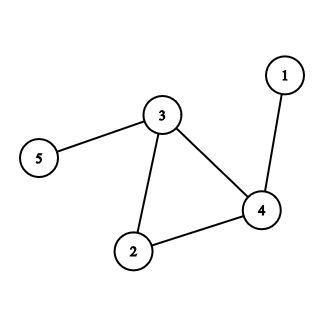
\includegraphics[width=0.5\textwidth]{unweighted_graph.png}
    \caption{Primer neusmerjenega grafa}
    \label{fig:mesh1}
\end{figure}

Zapis za graf na sliki je $G = (\{1, 2, 3, 4, 5\}, \{\{1, 4\}, \{4, 3\}, \{4, 2\}, \{3, 2\}, \{5, 3\}\})$

\subsubsection{Vozlišče}

Vozlišče je element množice V.

\subsubsection{Povezava}

Povezava je element množice E.

\subsubsection{Usmerjenost grafa}

Poznamo neusmerjene in usmerjene grafe. Za neusmerjen graf velja, da je povezava $v \in V$ množica moči dve, v kateri sta dve vozlišči. Za množice velja, da je $\{a, b\} = \{b, a\}$ (če velja, da je vozlišče a povezano z vozliščem b, je tudi vozlišče b povezano z vozliščem a). Pri usmerjenem grafu je povezava urejen par, za katerega velja $(a, b) \neq (b, a)$ iz tega sklepamo, da povezava $a \rightarrow b$ ni enaka $b \rightarrow a$ oziroma ni nujno, da nasprotna povezava v grafu sploh obstaja.

\begin{figure}[H]
    \centering
    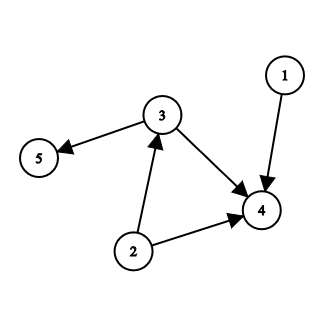
\includegraphics[width=0.5\textwidth]{directed_graph.png}
    \caption{Primer usmerjenega grafa}
    \label{fig:mesh1}
\end{figure}

\subsubsection{Obteženost grafa}

Vsak graf je lahko obtežen ali neobtežen. Če je graf obtežen, to pomeni, da lahko vsaki povezavi grafa določimo utež, vrednost ki ima lahko poljuben pomen, na primer dolžino med dvema točkama, ceno postavitve ceste med dvema mestoma, moč kovalentne vezi med dvema atomoma itd. . 

\subsubsection{Red grafa}

Red grafa G definiramo kot moč množice $V(G)$.

\subsubsection{Velikost grafa}

Velikost grafa G definiramo kot moč množice $E(G)$.


\subsubsection{Stopnja vozlišča}

Vozlišču $v \in V(G)$ lahko določimo stopnjo $deg(v)$, za katero v neusmerjenem grafu velja, da je enaka številu vseh sosednjih povezav.
\\ \\
V usmerjenem grafu lahko vsakemu vozlišču določimo vhodno in izhodno stopnjo. \textbf{Vhodna stopnja} vozlišča usmerjenega grafa $deg^+(v)$ nam pove število predhodnikov tega vozlišča oziroma število povezav v grafu, ki začnejo na poljubnem vozlišču in končajo v tem vozlišču, \textbf{izhodna stopnja} $deg^-(v)$ pa število njegovih naslednjikov oziroma število povezav ki začnejo v tem vozlišču.

\subsection{Podgraf}

Graf K je podgraf grafa G, če velja da je $K_V \subseteq G_V$ in $K_E \subseteq G_E$. 
\\ \\
\textbf{Vpet podgraf} grafa G je graf K, za katerega velja $K_V = G_V$ in $K_E \subseteq G_E$.

\subsubsection{Polni graf}

Polni graf je graf, v katerem obstaja povezava med katerimakoli različnima vozliščema.

\subsection{Minor}

Minor grafa G je graf M, do katerega pridemo, če na grafu G brišemo vozlišča, brišemo povezave ali krčimo povezave (zbrišemo povezavo med dvema vozliščema, nato pa obe vozlišči združimo v eno).

\subsection{Planaren graf}

Graf G je planaren, če ga je mogoče narisati na ravnino, brez da bi se katerekoli od povezav sekale. Wagnerjev izrek pravi, da je graf planaren če in samo če kot minorja ne vsebuje grafa $K_5$ (polnega grafa 5 vozlišč) ali grafa $K_{3, 3}$ (polnega dvodelnega grafa šestih vozlišč).

\begin{figure}[H]
    \centering
    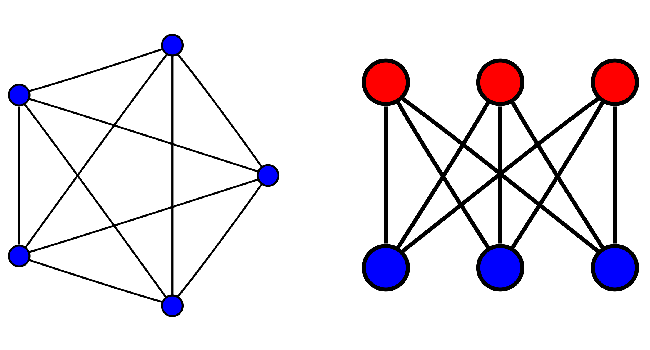
\includegraphics[width=0.5\textwidth]{k5_k33.png}
    \caption{grafa $K_5$ in $K_{3, 3}$}
    \label{fig:mesh1}
\end{figure}

\section{Implementacija grafa}

Graf lahko v računalniku predstavimo na vrsto različnih načinov, kjer ima vsak način svoje prednosti in slabosti. V tej raziskovalni nalogi sem se osredotočal predvsem na matriko sosednosti in seznam sosednosti, ki sta najpogostejša in najbolj generalna pristopa, vendar pa poznamo še vrsto drugih načinov, poleg tega pa lahko dodatno optimizacijo dosežemo tudi z kombiniranjem obeh pristopov.

\subsection{Matrika sosednosti}

Matrika sosednosti je eden najpogostejših pristopov k predstavitvi grafa. Osnovna ideja je, da za graf G določinmo matriko velikosti $n \times n$, kjer je n red grafa G in na vsako polje matrike $a_{ij}$ predstavimo relacijo med i-tim in j-tim vozliščem v grafu. Če je graf neobtežen lahko v matriko zapišemo 1 če povezava obstaja v nasprotnem primeru pa 0. V primeru obteženega grafa pa lahko lahko polje $a_{ij}$ predstavlja težo povezave med vozliščema i in j. Če je graf, ki ga predstavljamo neusmerjen, bo matrika simetrična. Matrika sosednosti omogoča, da v časovni zahtevnosti $O(1)$ dobimo relacijo med dvema vozliščima, vendar pa je prostorsko precej neučinkovita z zahtevnostjo $O(n^{2})$, ne glede na število povezav v grafu.

\[
	\begin{bmatrix}
		0 & 0 & 0 & 1 & 0 \\
		0 & 0 & 1 & 1 & 0 \\
		0 & 0 & 0 & 1 & 1 \\
		0 & 0 & 0 & 0 & 0 \\
		0 & 0 & 0 & 0 & 0 \\
	\end{bmatrix}
\]

\thickspace

\noindent
Primer matrike sosednosti za usmerjen graf na sliki 2. Ker graf na sliki ni povezan preveč gosto, ima večina polj matrike vrednost 0, kar je prostorsko potratno.


\subsection{Seznam sosednosti}

Seznam sosednosti za graf G je seznam dolžine reda G, ki na za vsako vozlišče grafa hrani vsa vozlišča, s katerimi je trenutno vozlišče povezano (v primeru obteženega grafa lahko poleg vozlišča hrani še težo povezave). Prednosti seznama sosednosti so, da je njegova prostorska zahtevnost $O(V+E)$, prav tako omogoča hitro iteracijo čez vse sosede nekega vozlišča. Slabosti seznama sosednosti pa so počasnejše preverjanje, ali povezava med dvema točkama obstaja in počasno brisanje povezav. Namesto seznama lahko v implementaciji uporabljamo tudi višje podatkovne strukture, na primer hash tabele, kar še dodatno pospeši delovanje.

\section{Osnovni algoritmi}

Kot del raziskovalne naloge sem napisal program, ki vizualizira delovanje nekaterih osnovnih algoritmov na neusmerjenem obteženem grafu.

\subsection{Preiskovanje v globino}
\subsection{Preiskovanje v širino}
\subsection{Boruvkov algoritem}
\subsection{Primov algoritem}

\section{Probemi teorije grafov}

\subsection{Barvanje grafov}
\subsection{Problem trgovskega potnika}

\subsection{Viri}


$https://en.wikipedia.org/wiki/Planar_graph$


\end{document}
